\documentclass{article}
\usepackage[utf8]{inputenc}
\usepackage[italian]{babel}
\usepackage{amsmath}
\usepackage{amssymb}
\usepackage{siunitx}
\usepackage{tabularray}
\usepackage{graphicx}
\usepackage{float}
\usepackage{xfrac}
\usepackage{caption}    % for \caption*{}
\newcommand*{\diam}{\varnothing}
\newcommand*{\best}[1]{{#1}_\text{best}}
\newcommand*{\bestp}[1]{{\left(#1\right)}_\text{best}}
\newcommand*{\pbest}[1]{\left({#1}_\text{best}\right)}
\newcommand*{\pbestp}[1]{\left({\left(#1\right)}_\text{best}\right)}
\newcommand*{\errrel}[1]{\frac{\delta #1}{{#1}_\text{best}}}
%% <custom footnotes/>
%\newcounter{savefootnote}
%\newcounter{symfootnote}
%\newcommand{\symfootnote}[1]{%
%   \setcounter{savefootnote}{\value{footnote}}%
%   \setcounter{footnote}{\value{symfootnote}}%
%   \ifnum\value{footnote}>8\setcounter{footnote}{0}\fi%
%   \let\oldthefootnote=\thefootnote%
%   \renewcommand{\thefootnote}{\fnsymbol{footnote}}%
%   \footnote{#1}%
%   \let\thefootnote=\oldthefootnote%
%   \setcounter{symfootnote}{\value{footnote}}%
%   \setcounter{footnote}{\value{savefootnote}}%
%}
%% </custom footnotes>
\title{
    Laboratorio di Fisica 1\\
    R8: Taratura di una termocoppia
}
\author{Gruppo 17: Bergamaschi Riccardo, Graiani Elia, Moglia Simone}
\date{30/04/2024 – 07/05/2024}
\makeindex
\begin{document}

\maketitle

\begin{abstract}
    Il gruppo di lavoro ha determinato la curva di calibrazione una termocoppia sfruttando
    punti fissi, ovvero temperature note, di alcune sostanze chimiche.
\end{abstract}

\setcounter{section}{-1}  % Count sections starting from 0
\section{Materiali e strumenti di misura utilizzati}
\begin{center}
    \begin{tblr}{
        width=\textwidth,
        colspec={ X[2,m,j]X[m,c]X[m,c]X[m,c] },
        vlines,
    }
        \hline
        \textbf{Strumento di misura} & \textbf{Soglia} & \textbf{Portata} & \textbf{Sensibilità} \\
        \hline
        Termocoppia (tipo K) & \qty{1?}{mV} & \qty{99999999?}{mV} & \qty{1}{mV} \\
        \hline
    \end{tblr}
    \begin{tblr}{
        width=\textwidth,
        colspec={ X[m,j]X[3,m,j] },
        vlines,
    }
        \hline
        \textbf{Altro} & \textbf{Descrizione/Note} \\
        \hline
        Sostanze chimiche & {
            Azoto, etanolo, ghiaccio,
            gallio, acqua e indio.
        } \\
        \hline[dashed]
        Fornelletto e pentolino & {
            Per scaldare i composti.
        } \\
        \hline
    \end{tblr}
\end{center}

\section{Esperienza e procedimento di misura}
\begin{enumerate}
    \item
        Immergiamo anche la seconda giunzione nel bagno
        di acqua e ghiaccio e leggiamo la ddp prodotta.
    \item
        Inseriamo la giunzione nel contenitore dell'azoto
        liquido ed osserviamo la ddp prodotta.
    \item
        Versiamo acqua distillata in un pentolino e la
        facciamo bollire; una volta raggiunto il bollore,
        inseriamo la giunzione nell'acqua per ricavare la ddp prodotta.
    \item
        Inseriamo nell'azoto liquido una provetta contenente
        etanolo liquido in modo da farlo solidificare:
        estratta la provetta, rileviamo la ddp quando
        l'etanolo fonde.
    \item
        Mettiamo il crogiolo di indio a scaldare a bagnomaria
        nel pentolino; una volta fuso vi inseriamo la giunzione
        ed lo facciamo raffreddare "naturalmente?", misurando
        la ddp durante la solidificazione.
    \item
        Facciamo fondere il gallio nel pentolino, per poi
        immergerlo nell'azoto liquido e scaldarlo nuovamente
        nel pentolino, leggendo la ddp durante la fusione.
    %facciamo questo perché:
    % -la temperatura di fusione del Ga è intorno ai 30°C, dunque esso si trovava spesso in uno stato intermedio tra due fasi
    % -bisogna evitare il fenomeno del sottoraffreddamento

\end{enumerate}

\section{Analisi dei dati raccolti e conclusioni}
\subsection{Calcolo del momento d'inerzia del campione}

Essendo il momento d'inerzia additivo, abbiamo calcolato
$I_\text{CM}$ sommando i singoli momenti d'inerzia rispetto al comune
asse di simmetria dei cilindri e dei tronchi di cono che compongono il
campione, dove la massa di ciascuno di essi è stata facilmente
calcolata assumendo la densità del campione uniforme.
Di seguito riportiamo tali misure:

\begin{table}[H]
    \centering

    \begin{tblr}{
        vlines = {},
        hline{1,2,17} = {},
        hline{3,5-7,9,10,12-14,16} = {dashed},
        cell{1,2,5,6,9,12,13,16}{1-5} = {c,m},
        cell{3,7,10,14}{1-3,5} = {r=2}{c,m},
    }
        $\#$&\emph{Forma}&$h\;(\unit{mm})$&$d_{1,2}\;(\unit{mm})$&$I\;(10^{-6}\;\unit{kg\,m^2})$\\
        1  & Cilindro          & $30.45\pm0.05$ & $49.90\pm0.05$ & $154.6 \pm1.8 $ \\
        2  & {Tronco\\di cono} & $ 5.95\pm0.10$ & $49.90\pm0.05$ & $ 13.7 \pm0.5 $ \\
           &                   &                & $29.40\pm0.05$ &                 \\
        3  & Cilindro          & $ 9.20\pm0.10$ & $25.85\pm0.05$ & $  3.36\pm0.08$ \\
        4  & Cilindro          & $10.80\pm0.05$ & $18.65\pm0.05$ & $  1.07\pm0.02$ \\
        5  & {Tronco\\di cono} & $ 4.25\pm0.05$ & $34.55\pm0.05$ & $ 11.8 \pm0.4 $ \\
           &                   &                & $49.90\pm0.05$ &                 \\
        6  & Cilindro          & $52.95\pm0.05$ & $49.90\pm0.05$ & $269   \pm3   $ \\
        7  & {Tronco\\di cono} & $ 4.25\pm0.05$ & $49.90\pm0.05$ & $ 12.6 \pm0.4 $ \\
           &                   &                & $36.35\pm0.05$ &                 \\
        8  & Cilindro          & $10.80\pm0.05$ & $18.75\pm0.05$ & $  1.09\pm0.02$ \\
        9  & Cilindro          & $ 9.25\pm0.10$ & $25.90\pm0.05$ & $  3.41\pm0.08$ \\
        10 & {Tronco\\di cono} & $ 5.95\pm0.10$ & $29.10\pm0.05$ & $ 13.5 \pm0.5 $ \\
           &                   &                & $49.90\pm0.05$ &                 \\
        11 & Cilindro          & $30.40\pm0.05$ & $49.90\pm0.05$ & $154.4 \pm1.8 $ \\
    \end{tblr}
\end{table}

\begin{itemize}
    \item Massa totale: $M=(2214.57\pm0.01)\;\unit{g}$
    \item Volume totale: $V=(2.654\pm0.017)\cdot10^{-4}\;\unit{m^3}$
    \item Densità media: $\rho=(8.34\pm0.05)\cdot10^{-3}\;\unit{kg \per m^3}$
    \item Momento d'inerzia totale: $I_\text{CM}=(6.38\pm0.09)\cdot10^{-4}\;\unit{kg\,m^2}$
\end{itemize}

\subsection{Distribuzione dei tempi di caduta}

Riportiamo di seguito i grafici della distribuzione dei tempi di caduta $t_{L,\theta}$,
accompagnati alle relative misure di $L$ e $\theta$.

\begin{center}
    %
\end{center}

\subsection{Calcolo di $g$ mediante la dinamica del corpo rigido}

Fissato un sistema di riferimento cartesiano ortogonale solidale
al piano inclinato, con origine nel punto di partenza del campione,
asse $x$ parallelo alle guide e asse $y$ entrante nel piano inclinato,
possiamo scrivere la legge del moto del centro di massa e le
equazioni cardinali della dinamica del corpo rigido:
\[x_\text{CM}(t) = \frac{1}{2} a_\text{CM} t^2\]
\[\left\{\begin{aligned}
    &M g \sin\theta - F_s = M a_\text{CM} \\
    &M g \cos\theta - F_n = 0 \\
    &R M g \sin\theta = \left(I_\text{CM} + M R^2\right) \alpha
\end{aligned}\right.\]
dove $R$ è il raggio di contatto, $\vec{F}_s$ è la forza di attrito statico
tra il campione e le guide, mentre $\vec{F}_n$ è la reazione vincolare delle
guide, normale al piano.

Per poter descrivere il moto del campione come di rotolamento puro,
dobbiamo assicurarci che $F_s \le \mu_s F_n$, con $\mu_s$ il
coefficiente di attrito statico tra il corpo rigido e le guide.
Se questa condizione è verificata, possiamo utilizzare la relazione:
\[\alpha = \frac{a_\text{CM}}{R}\]

Risolvendo il sistema lineare e la disequazione di cui sopra si ottiene:
\[\left\{\begin{aligned}
    &a_\text{CM} = \frac{M R^2}{I_\text{CM} + M R^2} g\sin\theta \\
    &F_n = M g \cos\theta \\
    &F_s = \frac{I}{I + M R^2} M g \sin\theta \\
    & 0 \le \alpha \le \arctan\left(\mu_s \left(\frac{MR^2}{I_\text{CM}} + 1\right)\right) \\
\end{aligned}\right.\]

Ricordando ora che $L = x_\text{CM}(\bar{t}_{L,\theta}) + D + S$, dove $D$ è il diametro
più esterno del campione e $S$ è lo spessore del cuscinetto, possiamo ricavare:
\[
    \frac{2(L-D-S)}{\sin\theta}\left(\frac{I_\text{CM}}{M R^2} + 1\right) = g \cdot \bar{t}_{L,\theta}^2
\]

Possiamo pertanto determinare il modulo di $\vec{g}$ mediante una regressione
lineare pesata\footnote{
    La scelta di una regressione lineare \emph{pesata} è giustificata dal fatto
    che gli errori sull'ascissa, per quanto ridotti, sono diversi fra di loro.
}:
\begin{figure}[H]
    % <v>^
    % 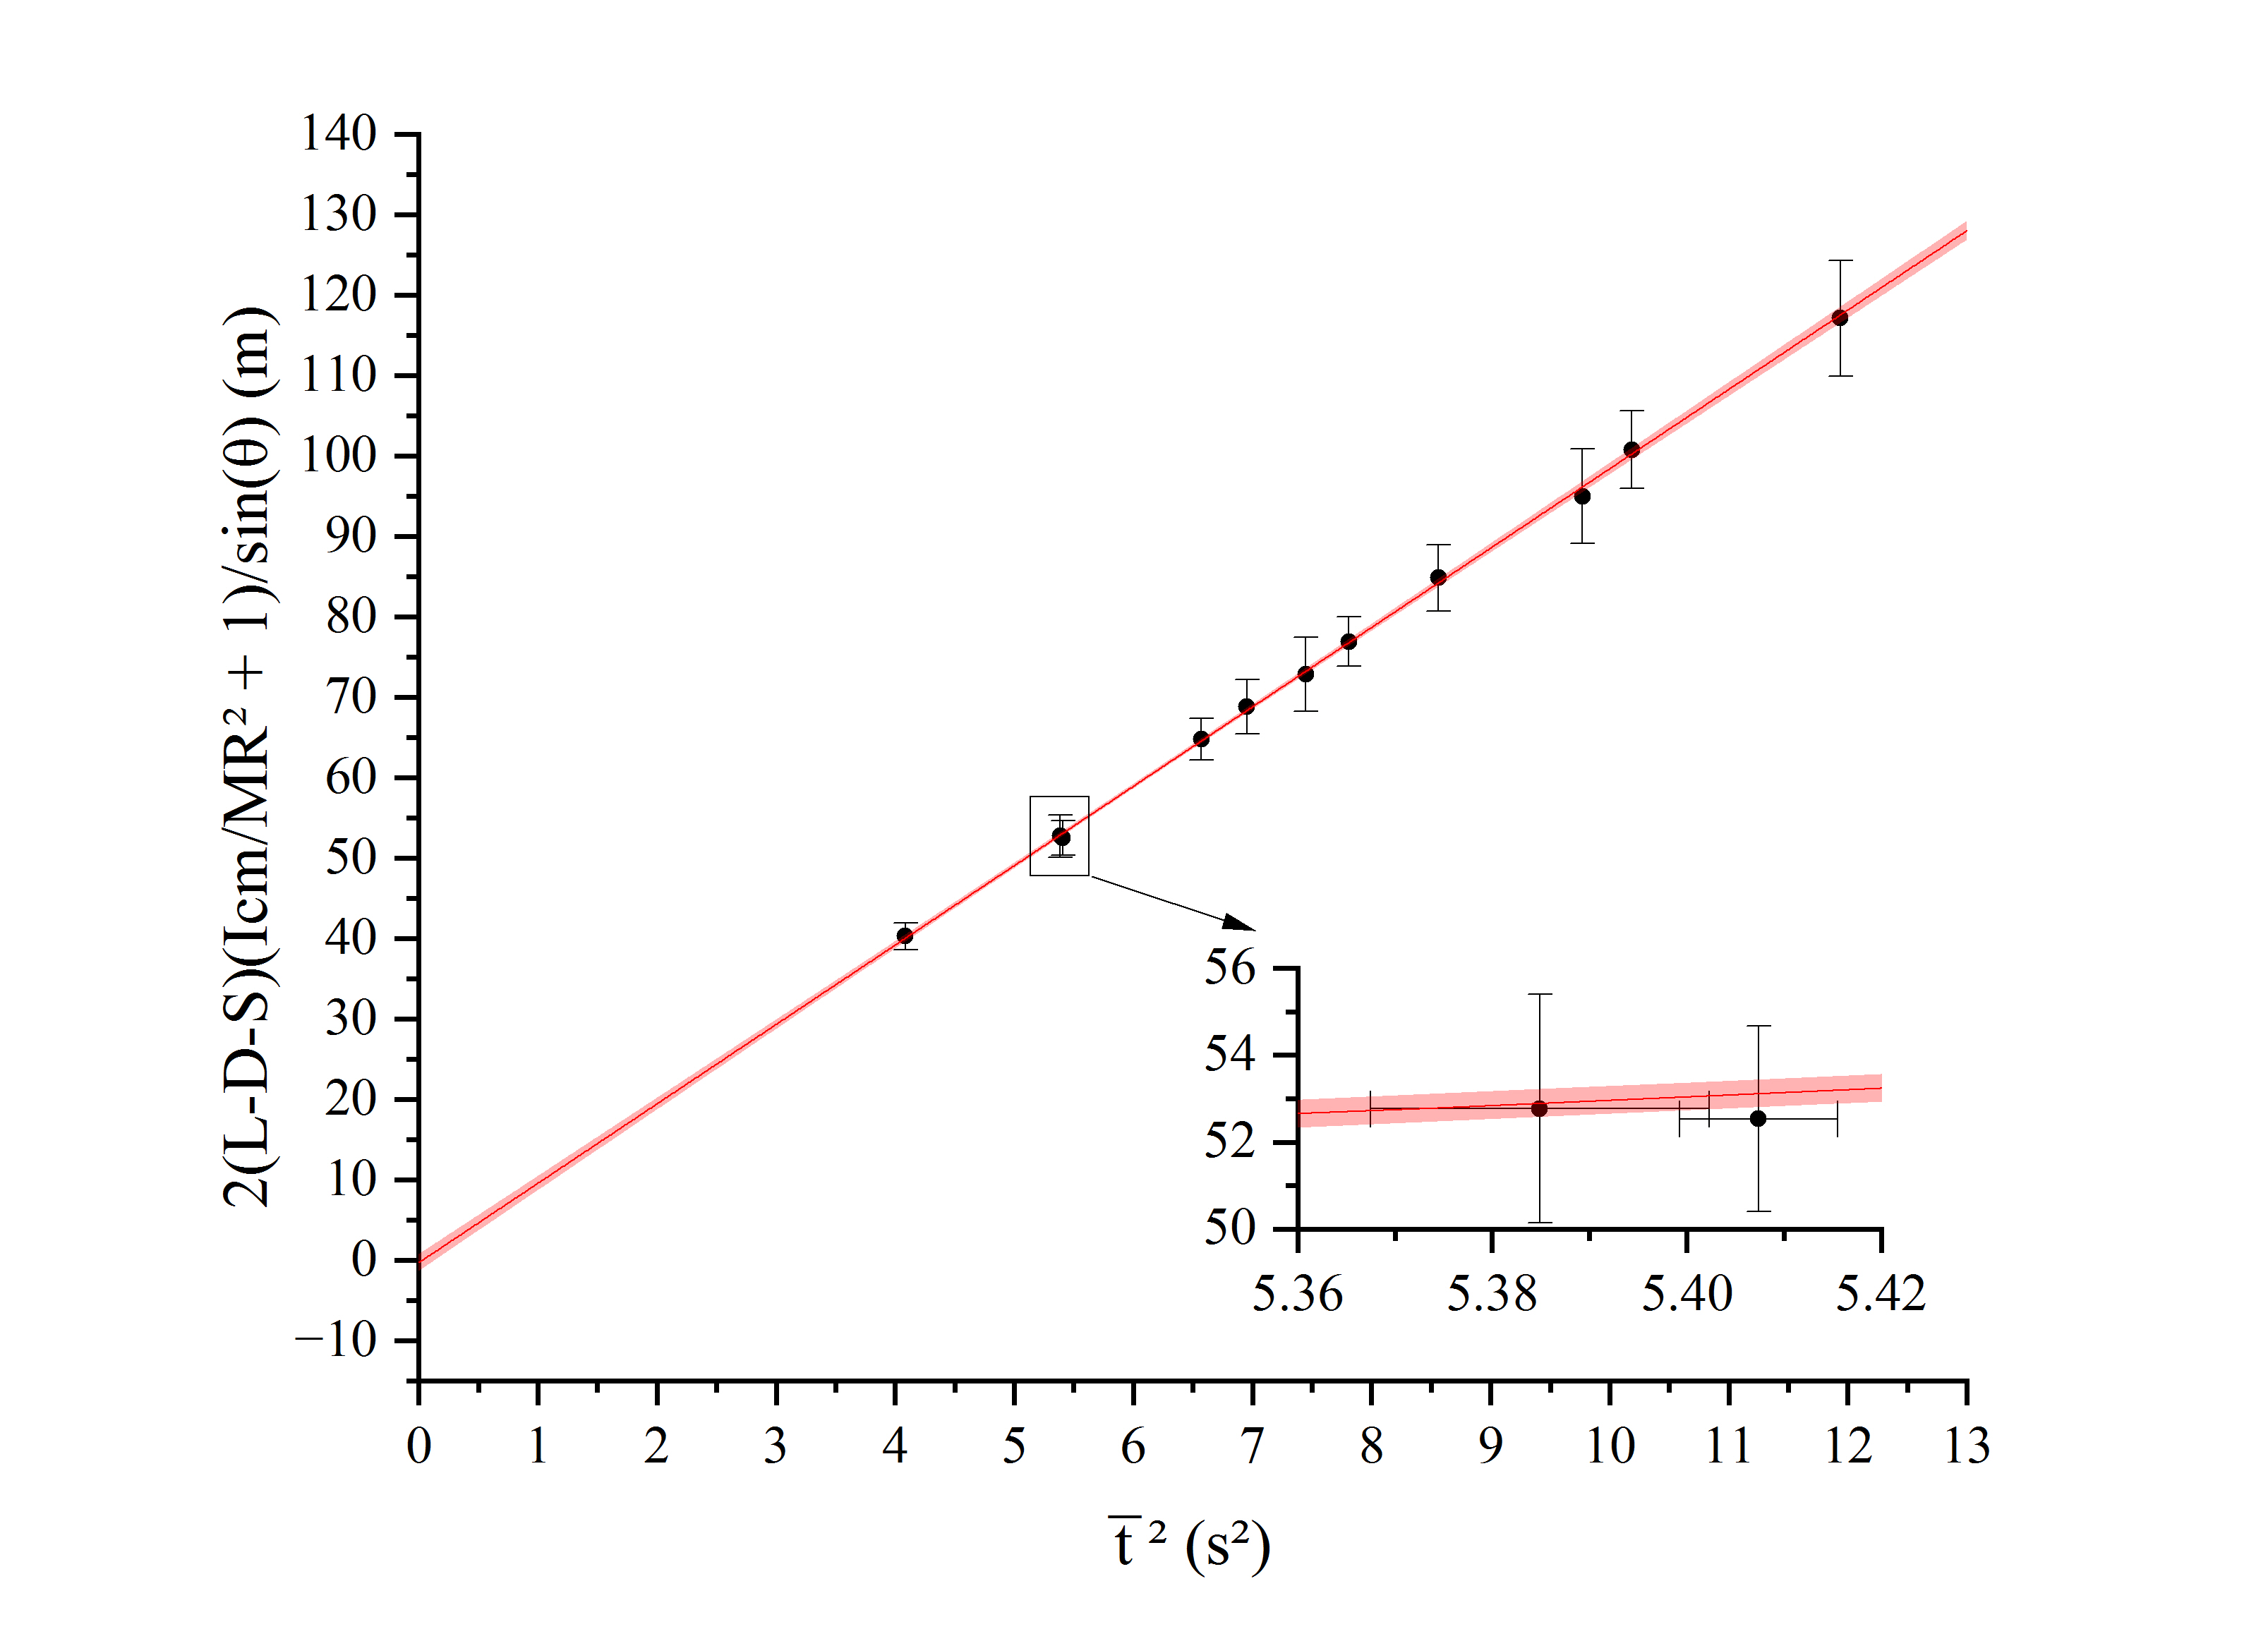
\includegraphics[trim={1cm 0.6cm 1cm 1cm},clip,width=\textwidth]{img/regressione.jpg}
    \caption*{\emph{
        In rosso la retta di regressione, in rosa la sua regione di incertezza. \\
        Nel grafico principale, le barre di errore lungo l'ascissa, date le loro
        dimensioni, non sono visibili.
    }}
\end{figure}

Di seguito riportiamo i risultati della regressione lineare:
\begin{itemize}
    \item Coefficiente angolare ($g$) $=(9.9\pm0.5)\;\unit{m \per s^2}$
    \item Intercetta $=(0\pm3)\;\unit{m}$ (compatibile con $0$, come ci si aspettava)
\end{itemize}

\end{document}
